
\subsection{Axial Shielding Factor Measurements}
In the first approach, the witness cylinder was used as a magnetic
shield.  The general idea is to measure any changes in the shielding
factor corresponding to a temperature change of the witness cylinder.
A solenoid producing a known homogeneous magnetic field was placed
outside the witness cylinder as shown in Fig.~\ref{fig:geometry}.  The
solenoid has 14 turns with XXX spacing between the wires. The radius
and the half length of the solenoid is 17.44~cm while the radius and
the half length of our most inner prototype passive shield is
18.44~cm. In this design, when the end caps of the innermost prototype
passive shield are on, the this solenoid can be approximated by an
infinite solenoid that produces a homogeneous magnetic field.  The
applied magnetic field was at the order of $\mu$T.  The solenoid
current was varied sinusoidally at typically 0.01 to 10~Hz.  A
Bartington fluxgate magnetometer XXX (model number) measured the
magnetic field at the center of the witness cylinder while the
temperature of the shield was measured.

% what was the solenoid field?  how homogeneous was the field?
% Discuss the coil design?  Typical coil current?
To increase the resolution of the measured signal from the fluxgate, a
Signal Conditioning Unit (SCU) with a low pass filter set to 10~Hz
(CHECK) and a gain set to typically 50 and higher was used. The
conversion factor for these fluxgates is 7~$\mu$T/V.  The signal from
the fluxgate was then demodulated by an SRS830 lock-in
% describe amplifier/filter of fluxgate (SCU), settings.
amplifier providing the in-phase and out-of-phase components of the
signal. The time constant on the lock-in was typically set to 3
seconds with 12~dB filter. The sensitivity settings was set by the
amplitude of the measured signal.
% describe the lock-in settings

\begin{figure}[h!]
\begin{center}
   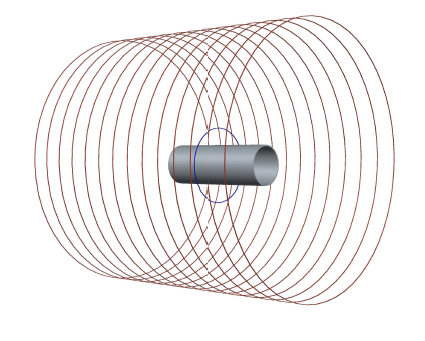
\includegraphics[width=0.8\textwidth]{geometry.PNG}
    \caption{This figure shows the setup of the axial shielding factor
      measurement. The witness cylinder with a radius of XXX and a
      length of XXX is placed inside a solenoid with a radius and a
      half length of 17.44~cm. The axis of symmetry is along the
      $z$-axis. The windings of the solenoid is shown in red. The blue
      coil with one turn is coupled to the witness cylinder and it has
      a radius of XXX.  }
    \label{fig:geometry}
    \end{center}
\end{figure}
% Add dimensions to figure.  Remove box and white space around
% diagram.

An example of the typical data acquired is shown in
Fig. \ref{fig:B_vs_Temp}. Graph (a) shows the temperature of the
witness cylinder over four days. The temperature changes are about
3.5~K and are caused by temperature variations of the room. The
magnetic field $B$ is the sum, in quadrature, of the in-phase and
out-of-phase components. For $f\lesssim 1$ Hz most of the measured
fluxgate signal is in the in-phase component. The magnetic field
tracks the temperature trend in an opposite way which is shown in
graph (b). The slope of the graph (c) has been calculated by using a
linear fit to the data. In general, we measured 0.3 \%/K $< \vert
\frac{1}{B} \frac{dB}{dT} \vert <$ 2.3 \%/K with the sign being
negative. The range also encompasses the typical deviation from a
linear $B(T)$ in the data (for example, those seen in
Fig.~\ref{fig:B_vs_Temp}(c).), and so we adopt this as an
uncertainty. Through a comprehensive set of systematic studies, the
source of the deviations from linearity could not be found. We suspect
it is due to a combination of mechanical stability and properties of
the material that cannot be embodied by a single temperature
slope. Thus the experiment tends to set a scale and sign for the
possible temperature dependence, rather than a value.
  \begin{figure}[h!]
\begin{center}
   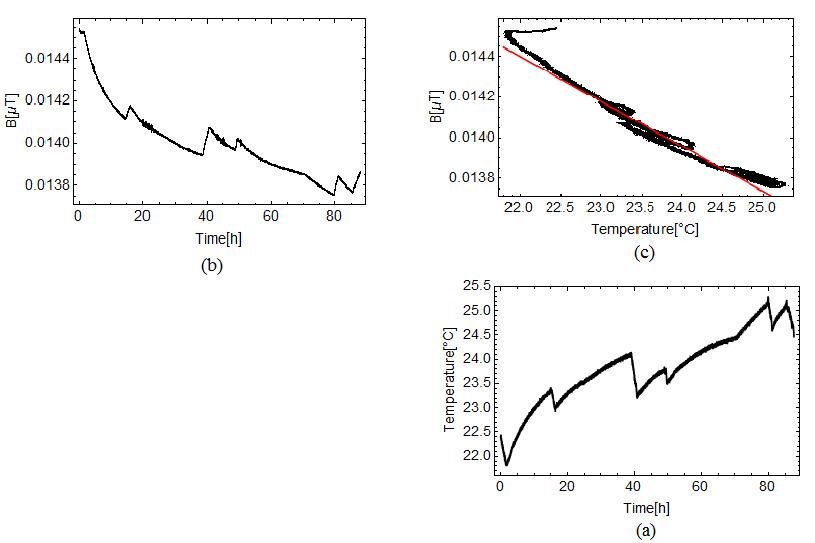
\includegraphics[width=0.5\textwidth]{B_vs_T.png}
    \caption{These graphs show data of temperature dependence of the
      magnetic field taken over 80 hours. Graph (a) shows the
      temperature of the witness cylinder in $^\circ$C as a function
      of time. Graph (b) shows the magnetic field inside the witness
      cylinder at the center in $\mu$T versus time and graph (c) shows
      the magnetic field in $\mu$T versus temperature in
      $^\circ$C. The red line is the linear fit to data. At
      22$^\circ$C, $\vert \frac{1}{B}\vert \vert
      \frac{dB}{dT}\vert\simeq -1.5 \% /K.$ }
    \label{fig:B_vs_Temp}
     \vspace{-2.em}
    \end{center}
\end{figure} 

To relate the data to $\mu(T)$, finite element simulations in FEMM and
OPERA were performed.  From these simulations the ratio $\frac{\mu}{B}
\frac{dB}{d\mu}$ was calculated in a model where $\bold{B}=\mu
\bold{H}$ and $\mu$ is a constant i.e. the material is treated as
being linear. The term $\frac{\mu}{B}\frac{dB}{d\mu}\neq 0$ because
the witness cylinders are open ended. Combining the measurement and
the simulations, the temperature dependence of effective $\mu$ (at
$\mu$=20000) can be calculated by
\begin{equation}
\frac{1}{\mu}\frac{d\mu}{dT}= -\frac{\frac{1}{B}\frac{dB}{dT}}{\frac{\mu}{B}\frac{dB}{d\mu}}.
\end{equation}

\subsubsection{Systematic Errors}

\paragraph{Initial Design}

%initial design stages
The initial design of the $\mu(T)$ measurement included Tygon tubing
wrapped around the witness cylinder in a spiral pattern to flow water
and change the temperature of the witness cylinder. In those
measurements, the amplitude of the signal was measured from a
Tektronix oscilloscope. The mechanical stability issues dominated the
systematic uncertainties. When water was running, the flexibility of
the tubing caused a movement in the witness cylinder. As an
alternative, the tubes were replaced by copper tubing. In this case,
the challenge was to create enough contact between the tubes and the
witness cylinder which was not successful. In another design, a TEC
was replaced with the tubing. The main issue with this design was that
it did not provide enough cooling for the witness cylinder and also it
was creating only local temperature changes on the witness
cylinder. In addition, despite of using heat sinks, the heat created
by the TEC itself made it very inefficient. To reduce the background
noise in this measurement, all the components interior to the
measurement volume should be non-magnetic. As a result, type T
thermocouples were used which has copper and constantan conductors.


% T-type are less magnetic than K-type.  How much less and what's the
% systematic error, since they are not nonmagnetic?  I would say it is
% unknown.  Is there a way to assign a number to this?
%Taraneh: I couldn't find any number associated to this. I am not sure if the fluxgates are sensetive enough to measure it too.

\paragraph{Final Design} 

%final design
The final design included the witness cylinder, which was placed with
a holder inside the innermost prototype passive shield. The
temperature variations of the witness cylinder was due to the
temperature changes in the room which was following the on and off
cycles of the building air conditioner. A Bartington magnetic field
sensor (fluxgate) was hold inside the witness cylinder at the centre
by plastic holder. The signal from the sensor was then demodulated by
an SRS830 lock-in amplifier. To convert the final measured voltage
from the sensor to $\mu$T, the sum in quadratures of the in-phase and
out of phase components of the lock-in amplifier was multiplied by the
scaling factor on the magnetic field sensor which is 7 $\mu$T/V.  The
mu-metal alloy has a thermal conductivity of 0.35
W/(cm$\cdot$K). Therefore, four thermocouples placed on different
spots on the witness cylinder to correct for small temperature
differences on each end of the witness cylinder.  In these
measurements, the farther side of the passive shields had the end caps
while the other side was left open to give access to the interior
region. Based on the magnetic field maps inside the passive shields,
for 10 $\mu$T applied magnetic field, the stability of the field was
to 0.1 $\mu$T level and the magnetic field was even more stable closer
to the closed side of the passive shields. Therefore the witness
cylinder was pushed to the side with the end caps on the passive
shields.

% Another list
% - amplitude measurement on oscilloscope (no lock-in). (done)
% - speed of temperature change? temperature homogeneity?  (not here yet) 
% - other methods of cooling and why they didn't work. (not here yet)(done)
% - magnetic contamination by thermocouples (done)

% The above list maybe explains other possible variations on the
% method that you tried that all seemed to have worse systematic
% errors.

% Then, a list of systematic errors once you settled on the final
% measurement technique...

% - field profile/homogeneity (done)
% - mechanical stability (done)
% - thermal expansion (done)
% - temperature dependence of fluxgate and SCU (done)
% - temperature dependence of lock-in (done)
% - temperature dependence of coil resistance (not here yet)
%    - Cupron/etc. study. plus
%    - measuring across the precision resistor
% - null measurement (Cu, and why it doesn't give the whole story, not here yet) (done)
% - effect of endcaps? (influence of external fields, not here yet)(done)
% - temperature dependence of reaction factor (negligible, not here yet)(done)
% - degaussing (not here yet)
% - measurements on different witness cylinders? (not here yet)(done)
% - vibrations of the building?(done)
% - ...
%
% Another list is on the oldelog somewhere.  Please find it.
% The above list is longer and inclusive of the old list.
% See oldelog entry 141 in Magnetic Fields.
%
% This list of systematics is addressed now...


To eliminate the coupling of the field profile and mechanical
stabilities, another coil was used which was coupled to the witness
cylinder as shown in Fig.~\ref{fig:geometry}.  This also enabled us to
study the dependence of the field profile to $\mu(T)$. The result of
this study did not show a significant change and data was similar to
Fig. \ref{fig:B_vs_Temp} (c). Therefore, the systematic error due to
the field profile is smaller than the unknown systematic errors of
Fig. \ref{fig:B_vs_Temp} and similar figures.
% What is the value of the systematic error deduced from this study?
% I would say that the result of this study was that we got similar
% data to Fig. 3(c).  Therefore the systematic error due to field
% profile is smaller than the unknown systematic error of Fig. 3(c)
% and similar figures.  also partly addresses possible changes in
% reaction factor with temperature. (done)


%Temperature dependence of fluxgate and SCU
In these measurements, a Mag-03IEL70 Bartington magnetic field sensor which has individual sensor elements and a Mag-03SCU signal conditioning unit were used.
The magnetic field sensor is a low noise sensor with a range of $\pm$70 $\mu$T and it has a scaling temperature coefficient of 15 ppm/K.


As another mechanical stability study, the movement of the Bartington
fluxgate flying lead due to thermal expansion was estimated. If the
fluxgate flying lead move about 1 mm normal to its axis of symmetry
which is parallel to the axis of the witness cylinder, the magnetic
field will change about 30~ppm/K over 20~K temperature changes.  The
thermal expansion of the mu-metal cylinder is at the order of
10~ppm/K~\cite{kruppvdm}.  An SRS830 lock-in amplifier has 50
ppm/K amplitude stability. It is documented in the operating
manual \cite{bib:lockin}.

%We did this for the transformer technique
The temperature dependence of the coil resistance was also measured by
measuring the voltage across a temperature controlled 1~$\Omega$
resistor.
%The results?

%Taraneh: I calculated from the long summary
The stability of the system was tested by replacing the mu-metal
witness cylinder with a similar copper cylinder. For all those
measurements the stability was $<0.1$\%/K. Although these type of
measurements help to find an error bar on the stability of the system
in general, they do not help to find the sources of the systematic
uncertainty.


%effect of the end caps
In this experiment, one side of our prototype passive shield was closed with the end caps while the other side left open for easier access to the interior region. The result of the magnetic field map inside the prototype shield when the solenoid was  turned on showed that closer to the far side of the shield, where the shield is closed, the magnetic field is more uniform. For a 10$\mu$T applied magnetic field the maximum change of the magnetic field along the axis of the passive shield was the order of 0.1~$\mu$T.
Therefore the witness cylinder was pushed to the far side of the prototype shield to reduce the non uniformity of the magnetic field.
%This is from oldElog entry 146: field map by Andrew Harrison

%temperature dependence of reaction factor
The changes in magnetic permeability has an effect on the measured magnetic field inside the witness cylinder. Since the reaction factor for this geometry is not strongly correlated to $/mu$ in Fig. \ref{fig:Magnetic_Field}, the changes of the magnetic field due to magnetic permeability changes in negligible. For XXX change in $\mu$ the magnetic field internal to the witness cylinder changes by XXX. 

%degaussing
The magnetization of the prototype passive shield changes the magnetic permeability of the material and so the reaction factor changes. The degaussing procedure has a considerable effect on the initial magnetic field.
%what next?

%different witness cylinders
Three witness cylinders were tested for these measurements. In most cases, despite keeping the conditions the same, the results were significantly different for each witness cylinder. The systematic studies could not address these sources of error. As a result these changes is believed to be driven by the intrinsic properties of the witness cylinders.   
In general, annealing process and take-out temperatures have a strong effect on the properties of the shields and so their $\mu$ value.
%vibration
Since the experiment site is located at the heart of downtown it is also possible that vibrations of the building affected the experiment setup and its machanical stability.

Although for most of the measurements the general trend of $B(T)$ graphs was consistent, the shape and positions of the nonlinear parts of $B-T$ graphs were changing.


% Two possibilities:

% 1. unknown systematic error(s)

% 2. complicated material properties that don't follow a straight line
% could depend on material history themselves.

% Therefore we state a range which should be indicative of the scale
% of possible temperature dependence.


Taking all these systematics into account, in this method it was found that 0.6\%/K
$\lesssim\frac{1}{\mu}\frac{d\mu}{dT}\lesssim 2.3\%$/K. 



%\begin{itemize}
%\item Describe experimental setup and important considerations
%  (e.g. relationship of data to effective $\mu$)
%\item Explain B, H, f, and dominant systematic effects.
%\item One figure of experimental setup?
%\item One data graph?
%\item State overall result and systematic error.
%\end{itemize}
